\section{XAML} 
\begin{frame}[fragile]{XAML}{Extensible Application Markup Language}
  %XAML is used extensively in .NET Framework 3.0 \& .NET Framework 4.0 technologies, particularly in Windows Presentation Foundation (or WPF)
  %Anything that is created or implemented in XAML can be expressed using a more traditional .NET language, such as C\# 
  \begin{itemize}
    \item .NET Framework
    \item Windows Presentation Foundation (WPF)
    \item XAML
    \begin{itemize}
      \item Bindings
      \item Styles \& Templates
      \item Commands
    \end{itemize}
    \item Model View ViewModel
  \end{itemize}


  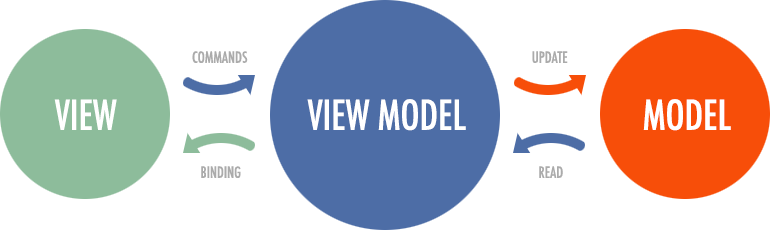
\includegraphics[width=\textwidth]{slides/mvvm.png}

\end{frame}

% Bindings to the viewmodel --------

\subsection{ViewModel Bindings} 
\begin{frame}[fragile]{XAML}{Properties in the ViewModel}

\begin{lstlisting}
<DatePicker SelectedDate="{Binding ActiveDate, Mode=TwoWay}" />
\end{lstlisting}

\begin{lstlisting}
public RecipeViewModel(Recipe recipe)
{
  ActiveDate = DateTime.Now;
  Recipe = recipe;
}

public Recipe Recipe { get; set; }

public DateTime ActiveDate
{
  get { return _activeDate; }
  set { _activeDate = value; }
}
\end{lstlisting}

\end{frame}

% BInding to the model ---------------

\subsection{Model Bindings} 
\begin{frame}[fragile]{XAML}{Properties in the Model}

\begin{lstlisting}
<Image Height="100" Width="100" Source="{Binding Recipe.Image}"/>
<Label Style="{StaticResource TextTitle}">
  <Label.Content>
      <AccessText Text="{Binding Recipe.Title}"/>
  </Label.Content>
</Label>
<ScrollViewer>
  <TextBlock Text="{Binding Recipe.RecipesPreparation.Preparation}" TextWrapping="Wrap"/>
</ScrollViewer>
\end{lstlisting}

\begin{lstlisting}
public partial class Recipe
{
  public int ID { get; set; }
  public string Title { get; set; }
  public int Persons { get; set; }
  public string Image { get; set; }
  public virtual ObservableCollection<RecipeIngredient> RecipeIngredients { get; set; }
  public virtual RecipesPreparation RecipesPreparation { get; set; }
}
\end{lstlisting}

\end{frame}


% ------------------ Styles and termplates ---------------------
\subsection{Styles and Templates} 
\begin{frame}[fragile]{XAML}{Styles \& Templates}
Styles
\begin{lstlisting}
<Style TargetType="{x:Type Control}" x:Key="TextTitle">
  <Setter Property="Foreground" Value="{StaticResource Text.Orange}"/>
  <Setter Property="FontSize" Value="14"/>
</Style>

<Style x:Key="DateLabelTemplate" TargetType="{x:Type Label}" BasedOn="{StaticResource TextLabelTemplate}">
    <Setter Property="ContentStringFormat" Value="dddd&#x0a;dd/MM"/>
</Style>
\end{lstlisting}

\end{frame}

\begin{frame}[fragile]{XAML}{Styles \& Templates}
Templates
\begin{lstlisting}
<DataTemplate x:Key="ListRecipesTemplate">
  <Grid>
    <Border Name="ItemBorder" Margin="3" BorderBrush="{StaticResource Button.Static.Border}" BorderThickness="1">
      <Grid Name="ItemGrid">
        <Image Height="75" Width="75" Stretch="UniformToFill" Source="{Binding recipe.Image}" />
        <Label Content="{Binding getMatchPercentage}" ContentStringFormat=" {0} ingredients"/>
        <TextBlock Text="{Binding recipe.Title}" TextTrimming="CharacterEllipsis" Style="{StaticResource TextblockTitle}" FontSize="20"/>
      </Grid>
    </Border>
  </Grid>
</DataTemplate>
\end{lstlisting}
\end{frame}


% --------------- COMMANDS ------------

\subsection{Commands} 
\begin{frame}[fragile]{XAML}{Navigation Commands}
%Hvad er commands...

\begin{lstlisting}
<Button Command="{Binding RemoveMealCommand}" Visibility="{Binding isMealSet}" Style="{StaticResource ButtonIconTemplate}>
    <Button.Background>
      <ImageBrush ImageSource="../Images/minusIcon.png" Stretch="Uniform"/>
    </Button.Background>
</Button>
\end{lstlisting}

\begin{lstlisting}
public ICommand RemoveMealCommand {
  get {
    if (_removeMealCommand == null) {
      _removeMealCommand = new RelayCommand(() => RemoveMeal());
    }
    return _removeMealCommand;
  }
}
\end{lstlisting}
\end{frame}


% navigat-or/ion commands
\begin{frame}[fragile]{XAML}{Commands}
%Section of \textit{<DataTemplate x:Key="MealsListBoxTemplate">}
\begin{lstlisting}
  <i:Interaction.Triggers>
    <i:EventTrigger EventName="MouseUp">
      <i:InvokeCommandAction Command="{Binding Source={x:Static local:Navigator.GoToRecipeFromMealCommand}}" CommandParameter="{Binding Content, RelativeSource={RelativeSource AncestorType={x:Type ListBoxItem}}}" />
    </i:EventTrigger>
  </i:Interaction.Triggers>
\end{lstlisting}

\begin{lstlisting}
public static ICommand GoToRecipeCommand {
  get {
    if (_goToRecipeCommand == null) {
      _goToRecipeCommand = new RelayCommand<Recipe>(recipe => {
        RecipeViewModel rvm = new RecipeViewModel(recipe);
        RecipePage rp = new RecipePage();
        rp.DataContext = rvm;
        Navigator.Navigate(rp);
      });
    }
    return _goToRecipeCommand;
  }
}
\end{lstlisting}
\end{frame}
